\documentclass{article}
\usepackage[a4paper,left=3.5cm,right=2.5cm,top=2.5cm,bottom=2.5cm]{geometry}
%%\usepackage[MeX]{polski}
\usepackage[cp1250]{inputenc}
\usepackage{polski}
%%\usepackage[utf8]{inputenc}
\usepackage[pdftex]{hyperref}
\usepackage{makeidx}
\usepackage[tableposition=top]{caption}
\usepackage{algorithmic}
\usepackage{graphicx}
\usepackage{enumerate}
\usepackage{multirow}
\usepackage{amsmath} %pakiet matematyczny
\usepackage{amssymb} %pakiet dodatkowych symboli
%\usepackage{colortbl}
\usepackage[table]{xcolor} % pakiet kolor�w
\begin{document}
	\begin{table}
		\centering
			\begin{tabular}{c|c|c}
				\hline\hline
					$x_{1}$ & $x_{2}$ & $( x_{1} \text{AND} x_{2} )$ \\ \hline
					1 & 1 & 1 \\
					1 & 0 & 0 \\
					0 & 1 & 0 \\
					0 & 0 & 0 \\
					\hline	
					\hline
			\end{tabular}
			\caption{Praca Domowa-Tabela 11}
			\label{tab: 1}
	\end{table}
	\begin{table}
		\centering
			\begin{tabular}{|r|l|}
				\hline
					7C0 & hexadecimal \\
					3700 & octal \\ \cline{2-2}
					11111000000 & binary \\
					\hline \hline
					1984 & decimal \\
					\hline
			\end{tabular}
		\caption{Praca Domowa-Tabela bez podpisu}
		\label{tab: 2}
	\end{table}	
	\begin{table}
		\centering
			\begin{tabular}{|c|c|c|c|c|c|c|c c}
				\cline{4-7}
					\multicolumn{3}{c|}{} & \multicolumn{4}{|c|}{Primes} \\ \cline{4-7}
					\multicolumn{3}{c|}{} & 2 & 3 & 5 & 7 \\ \cline{1-7}
					\multirow{2}{*}{Powers} & \multicolumn{2}{c|}{504} & 3 & 2 & 0 & 1  \\ \cline{2-7}
																	& \multicolumn{2}{c|}{540} & 2 & 3 & 1 & 0  \\ \cline{1-7}
					\multirow{2}{*}{Powers} & \multicolumn{2}{c|}{gcd} & 2 & 2 & 0 & 0 & min \\ \cline{2-7}
																	& \multicolumn{2}{c|}{lcm} & 3 & 3 & 1 & 1 & max \\ \cline{1-7}
			\end{tabular}
		\caption{Praca Domowa-Tabela 15}
		\label{tab: 3}
	\end{table}	
	\begin{table}
		\centering
		\rowcolors{1}{red}{pink}
			\begin{tabular}{ccc}
				czerwony & 1 & 2 \\ 
				r�?owy & 1 & 2 \\ 
				czerwony & 1 & 2 \\
				r�?owy & 1 & 2 \\
			\end{tabular}
		\caption{Praca Domowa-kolorowa}
		\label{tab: 4}
	\end{table}
	\begin{figure}[h!]
		\caption{A picture of a gull.}
		\centering
		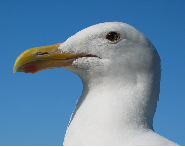
\includegraphics[width=0.5\textwidth]{gull.png}
	\end{figure}
	\begin{figure}[h!]
		\caption{A picture of the same gull looking the other way!}
		\centering
		\reflectbox{%
		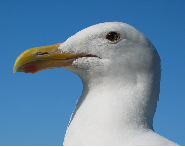
\includegraphics[width=0.5\textwidth]{gull.png}
		}
	\end{figure}
	\begin{figure}[h!]
		\centering
		\caption{Wy?wietlanie wielu obrazk�w jednocze?nie.}
			\reflectbox{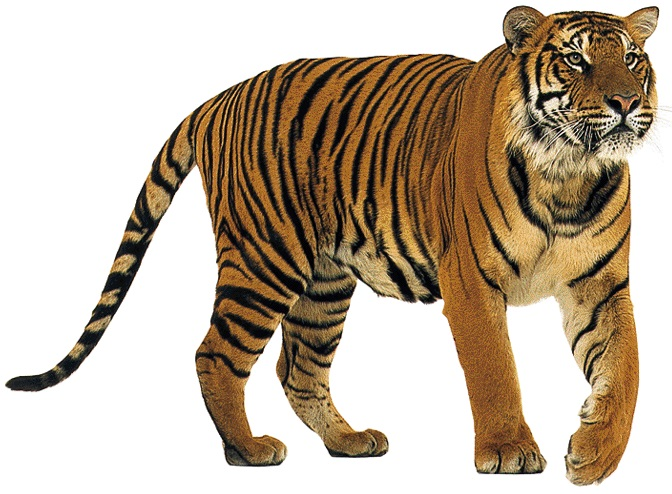
\includegraphics[scale=0.1]{tygrys.jpg}}
			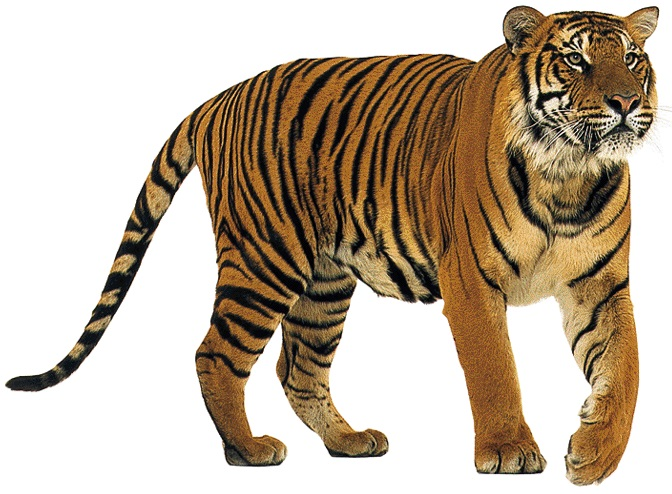
\includegraphics[scale=0.15]{tygrys.jpg}
			\reflectbox{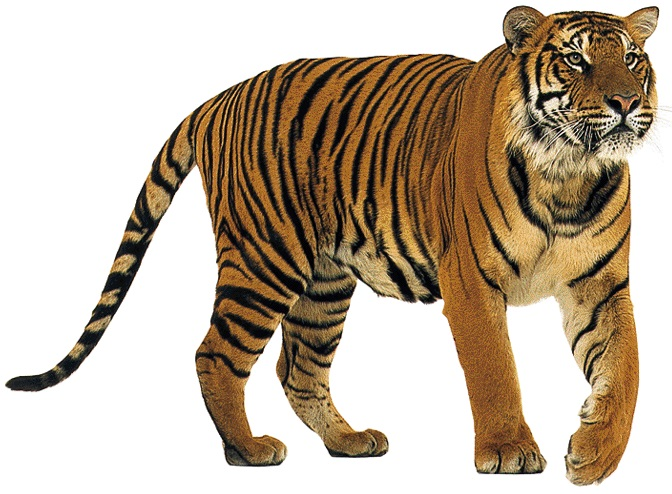
\includegraphics[scale=0.2]{tygrys.jpg}}
			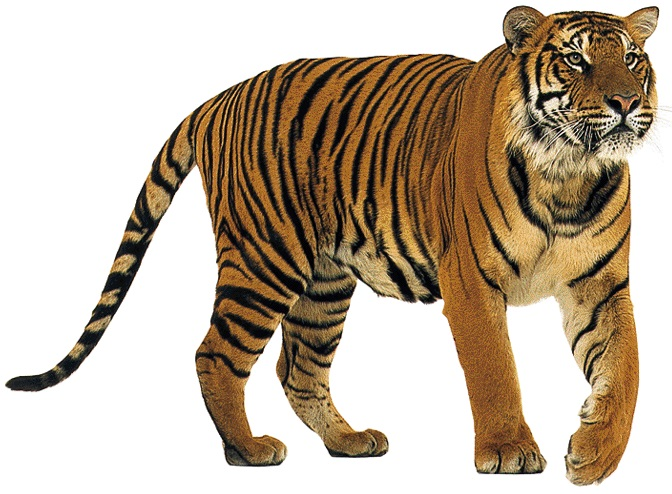
\includegraphics[scale=0.3]{tygrys.jpg}
	\end{figure}
\end{document}